\startchapter{Capturing the Latent Feature of Power Devices}
\label{chap:latentF}
\section{Introduction}
The objective of this work is to reduce the cost of power quality monitoring by intelligently placing power quality meters on selected links in the power network. After deploying limited number of meters, we should be able to estimate the power quality (PQ) values on unmonitored links as accurately as possible. A candidate link for meter placement is the one whose power quality is the most uncertain. The challenge here is how to identify the most uncertain links. Clearly, the PQ values on any power link is dependent on the physical characteristics of the electric devices. For example, the power quality at the output link of a UPS is more predictable than that of a switch. Hence, we need to know the behavior of each device in the network. We call the behavior of a device its latent feature or simply a transition function, which is usually estimated through physical modeling or through the assessment of historical power monitoring data.

In this chapter, we first introduce a latent feature model to capture the behavior of electric devices in the power network. Using a real power quality dataset, we then demonstrate that the historical data can be used to capture the latent features of a device. We use $k$-fold cross-validation technique to measure the accuracy of latent features we obtain using our dataset. Experimental evaluations show that the captured latent features are consistent. The latent features (or transition functions) are then used to propose our meter placement algorithms.

\begin{figure}[!t]
\center
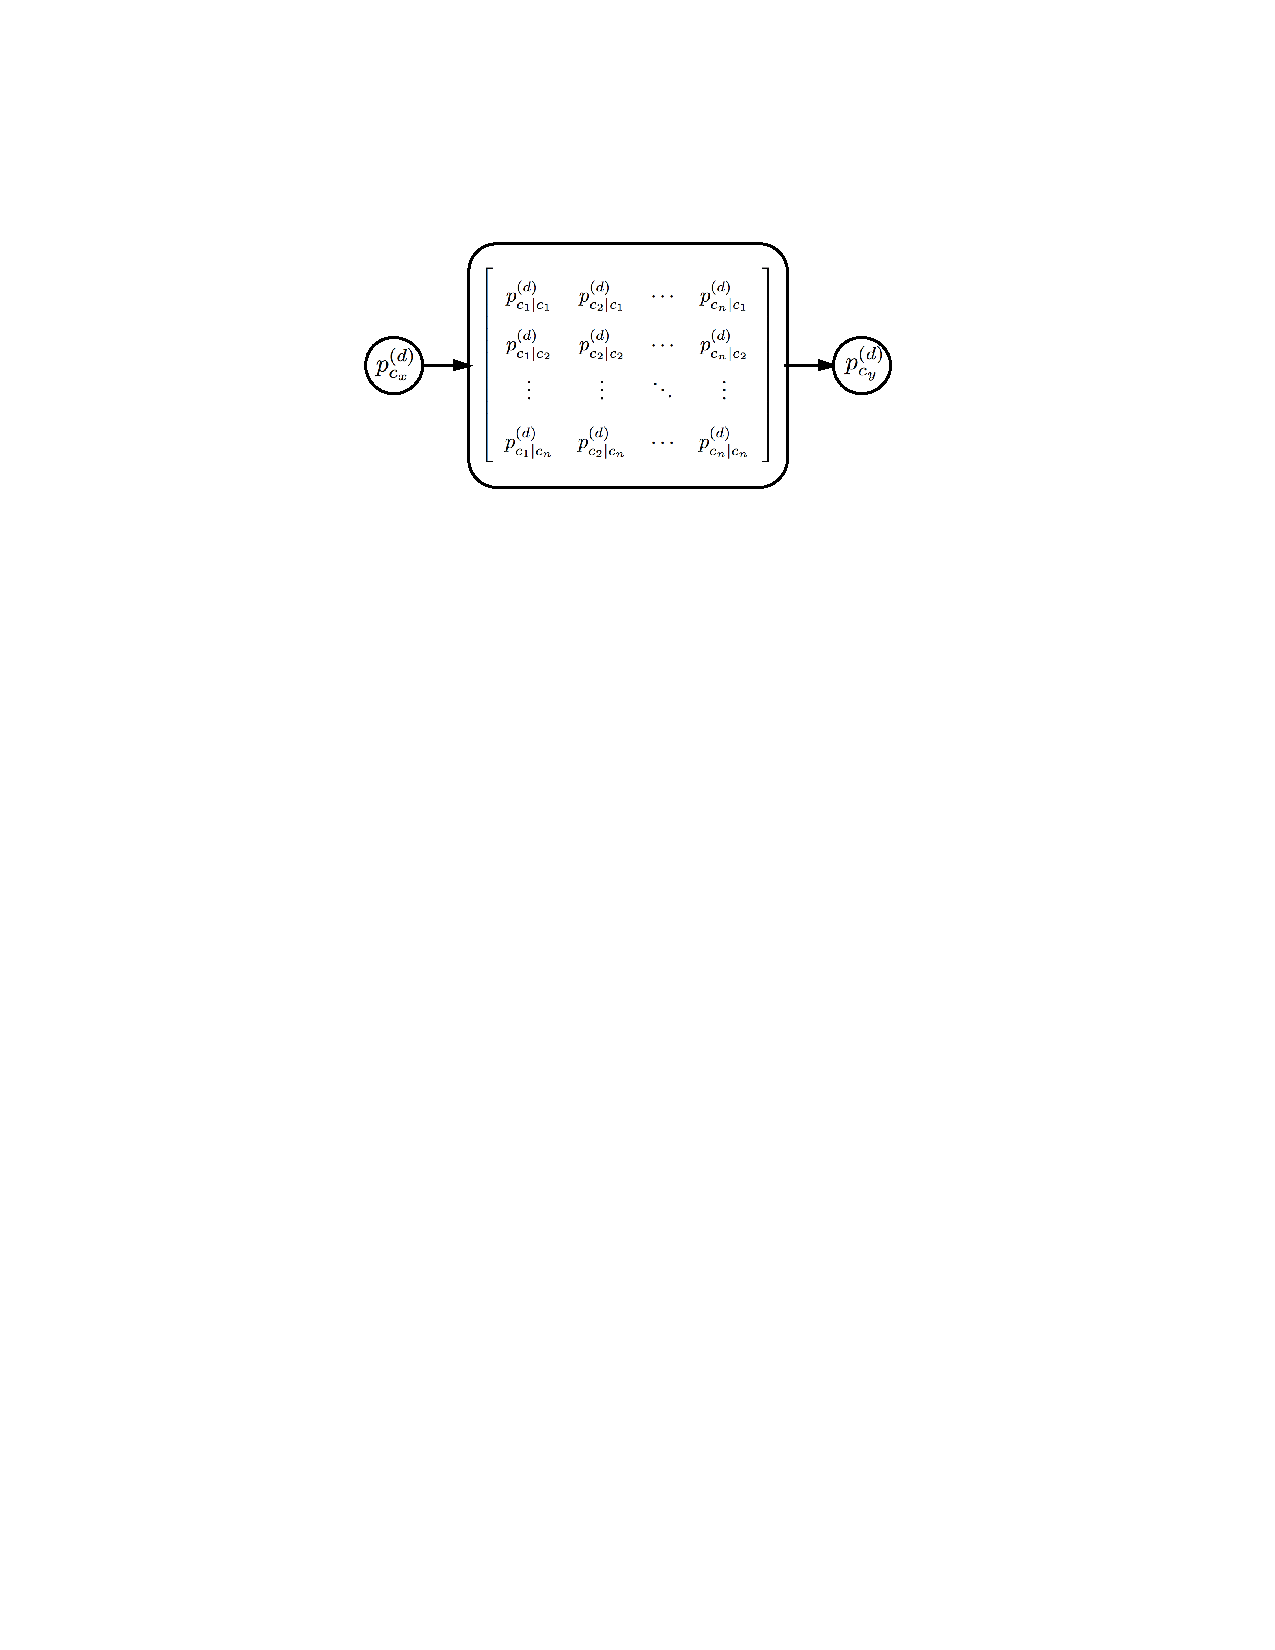
\includegraphics[width=0.75\columnwidth]{latentModel}
\caption{Latent feature model of a device $d$ where the two circles represent the power quality meters at input and output of node $d$; the matrix inside the node $d$ represents the transition function of the node.}
\label{fig:latentModel}

\end{figure}

\begin{figure}[!t]
\center
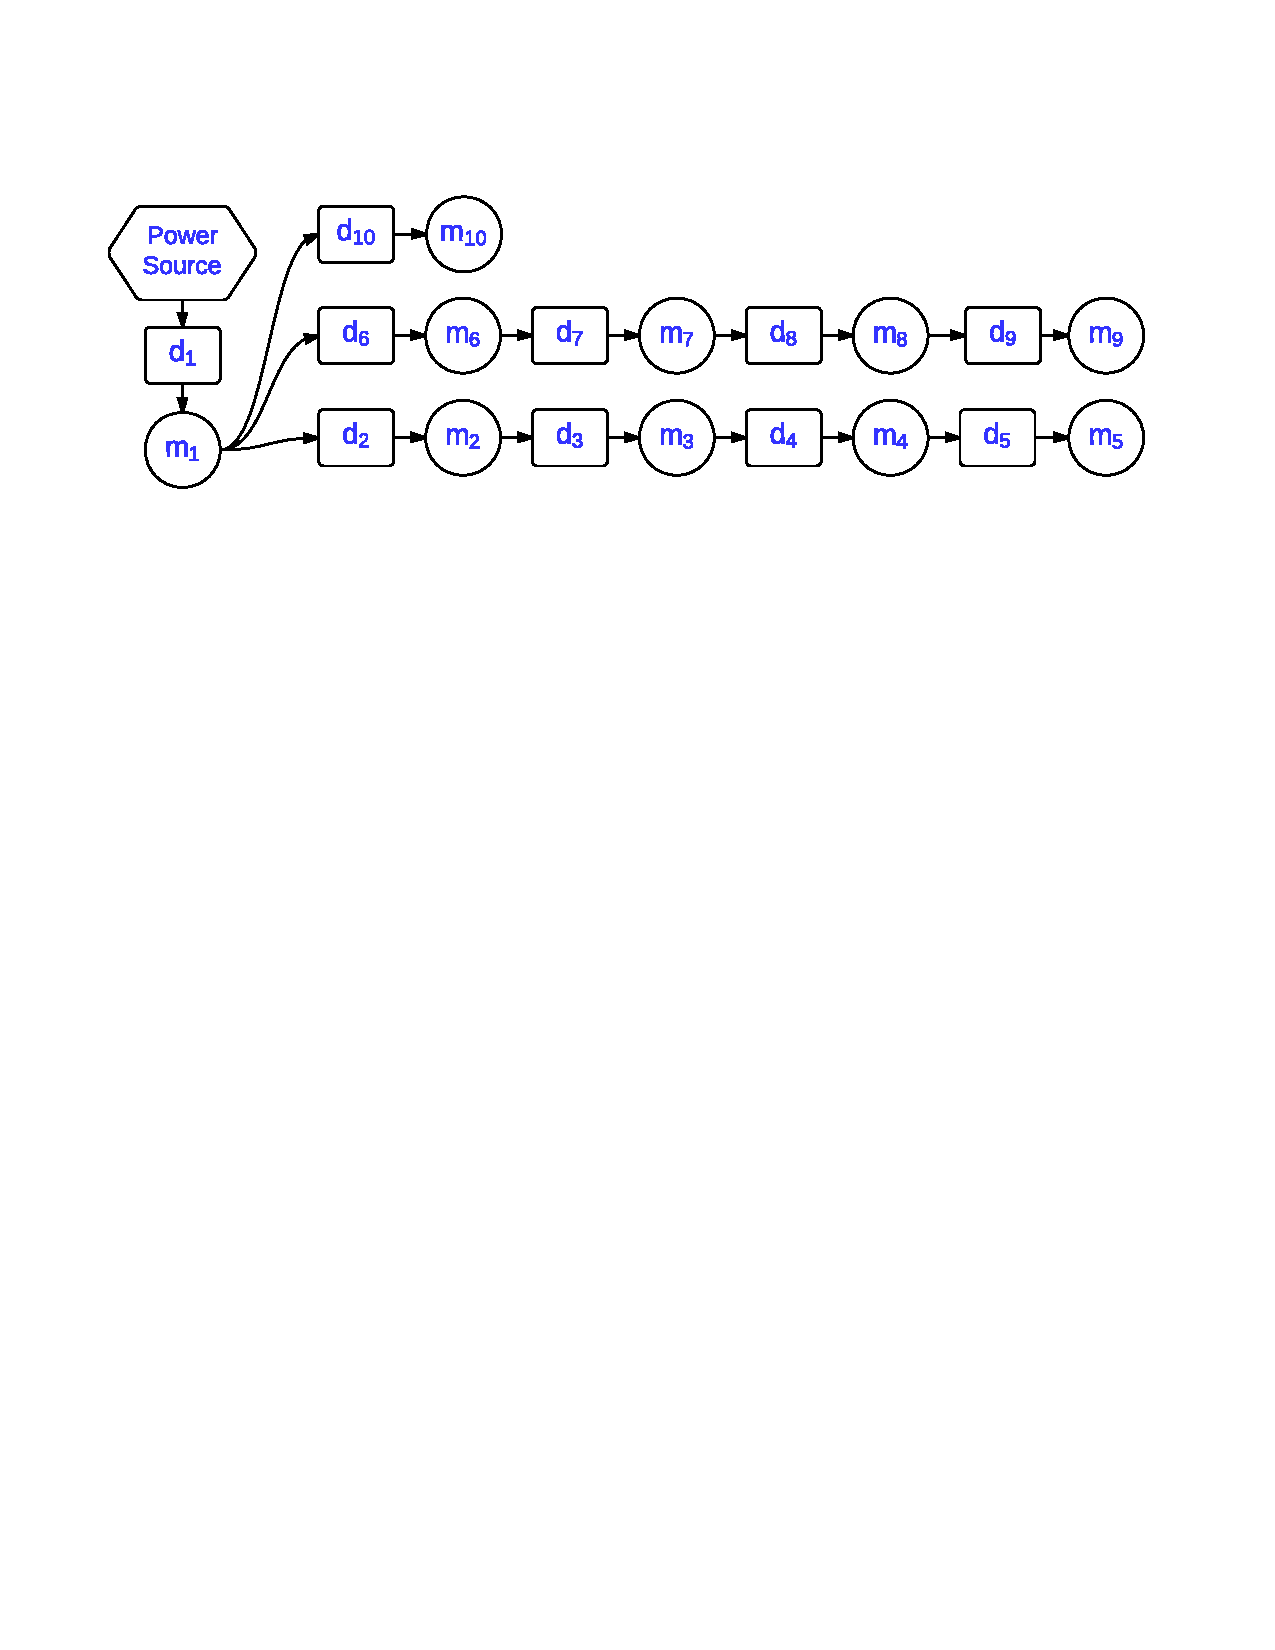
\includegraphics[width=0.98\columnwidth]{pqeNetwork}
\caption{Graph network of power quality meters installed in a power network.}
\label{fig:pqeNetwork}
\end{figure}

\section{The Latent Feature Model}
The latent feature model is basically a mechanism for capturing and mathematically representing the behavior of a device. We capture this behavior by monitoring the input and output links of electric devices and representing it as a transition function. A transition function ($f(d)$) of a device $d$ is the matrix consisting of real values representing the probabilities that a power quality input $c_x$ is mapped to another power quality $c_y$ at the output link of a device $d$. Figure~\ref{fig:latentModel} shows the proposed latent feature model we use to capture $f(d)$. We use a real-world power quality dataset collected for a period of over 4 years to capture the latent features of various electric devices. The latent feature $f(d)$ is then used to probabilistically estimate the power quality at unmonitored power links in the power network.

\section{Power Quality Dataset}
Our power quality dataset was collected at an enterprise power network for a period of four years. For privacy and security reasons, the physical network structure/diagram is omitted. Instead, we represent the topology/positions of the installed power quality meters via a graph network as shown in Fig.~\ref{fig:pqeNetwork}. There are a total of $10$ power quality meters (numbered from $m_1$ to $m_{10}$) installed. Each meter reported the power quality events (sag/swell, transient, etc.) to the data collection server via Ethernet network. It is important to mention that we currently do not consider transmission network, but only focus on power distribution network at the enterprise-level, e.g., university campus. Hence, we collect the power quality dataset at an enterprise network located at the distribution level. The network is using a standard three-phase distribution system. Devices of varying loads are using this network, including electric vehicles and large motors. Three-phase transformers with four-wire output are used for $120$ volt service. Table~\ref{tbl:perDevFreq} shows the number of events reported by each power quality meter while the positions of the meters are shown in Fig.~\ref{fig:pqeNetwork}.

\begin{table*}[!t]
\caption{Frequency table showing the number of events generated/reported by each power quality meter.}
\centering 
\renewcommand{\tabcolsep}{0.15cm}
\begin{tabular}{|c|c|c|c|c|c|c|c|c|c|c|}
\hline Meter ID & 1 & 2 & 3 & 4 & 5 & 6 & 7 & 8 & 9 & 10\tabularnewline
\hline No. of Events & 1705 & 629 & 756 & 764 & 777 & 282 & 309 & 181 & 44 & 657\tabularnewline
\hline 
\end{tabular}
\label{tbl:perDevFreq}
\end{table*}

\begin{table*}[!t]
\caption{Frequency table showing the number of events classified as IEEE power quality class ($c_i$).}
\centering 
\renewcommand{\tabcolsep}{0.12cm}
\begin{tabular}{|c|c|c|c|c|c|c|c|c|c|c|c|c|c|c|}
\hline Power Quality Class & $c_1$ & $c_2$ & $c_3$ & $c_4$ & $c_5$ & $c_6$ & $c_7$ & $c_8$ & $c_9$ & $c_{10}$ & $c_{11}$ & $c_{12}$ & $c_{13}$ & $c_{14}$\tabularnewline
\hline Number of Events & 3056 & 738 & 1485 & 274 & 144 & 354 & 10 & 11 & 0 & 2 & 8 & 2 & 19 & 1\tabularnewline
\hline 
\end{tabular}
\label{tbl:perClassFreq}
\end{table*}

The original power quality events reported by our power quality meters carry detailed information where some of the reported attributes are not directly relevant to power quality monitoring. For instance, we have a large number of branch circuit monitors installed that log every 15 minutes. Second, due to the detailed information content, the size of the raw dataset was about $40$ GB. In order to simplify the format and make the dataset concise and easy to analyze, we transform the reported events into a tabular form consisting of the power quality attributes we used. As a result, there are about $6000$ power quality events recorded in the dataset. Sample events from the dataset are shown in Table~\ref{tbl:sampleData}.

\begin{table}[!t]
\caption{Sample events from the dataset collected.}
\centering 
\renewcommand{\tabcolsep}{0.18cm}
\begin{tabular}{|c|c|c|c|c|c|c|}
\hline  \specialcell{Event\\ID} & \specialcell{Node\\ID} & \specialcell{Duration\\(seconds)} & \specialcell{Magnitude\\(volts)} & Severity  & Phase & Type\tabularnewline
\hline 119 & 5 & 0.02 & 292	& 3.19  & V1 &  Transient\tabularnewline
 338 & 6 & 1.002 & 147 & 47.1 & V2 & Swell\tabularnewline
 763 & 1 & 0.07 & 84.4 & 1.03  & V3 & Sag\tabularnewline
\hline 
\end{tabular}
\label{tbl:sampleData}
\end{table}

\begin{enumerate}
\item Each row in the table represents a power quality event.
\item The magnitude field represents a percentage of the nominal voltage that the sag or swell reached at its maximum (for instance the number $84$ means that voltage is sagged to $84\%$ of its nominal value, $147$ means that it swelled up by $47\%$ over its nominal value).
\item The severity field is a calculated statistic that combines the magnitude, duration and class of an event to provide a ranking variable.
\end{enumerate}

\begin{table}[!t]
\caption{Sample events classification using IEEE Standard 1159~\cite{IEEE09_1159}.}
%\vspace{-0.1in} 
\centering 
\begin{tabular}{|c|c|c|c|c|}
\hline \specialcell{Node\\ID} & Start Time & \specialcell{Duration\\(seconds)} & \specialcell{Magnitude\\(volts)} & IEEE Event Class\tabularnewline
\hline 4 & 733051.9385 & 0.00065 & 127 & $c_1$\tabularnewline
 4 & 733052.9522 & 0.00754 & 146 & $c_2$\tabularnewline
 8 & 733452.0117 & 0.00013 & 132 & $c_1$\tabularnewline
 7 & 733462.7471 & 0.049 & 84 & $c_3$\tabularnewline
 6 & 733488.8235 & 1.002 & 147 & $c_7$\tabularnewline
 6 & 733569.0525 & 0.518 & 79 & $c_6$\tabularnewline
 1 & 733572.9232 & 0.001 & 131 & $c_1$\tabularnewline
 7 & 733589.9307 & 0.016 & 82 & $c_3$\tabularnewline
 6 & 733724.0312 & 7105.48 & 30 & $c_{12}$\tabularnewline
 3 & 733724.1134 & 0.01664 & 233 & $c_4$\tabularnewline
\hline 
\end{tabular}
\label{tbl:sampleClassData}
\end{table}

Using IEEE Standard 1159~\cite{IEEE09_1159}, we classify the power quality events based on the fluctuation of the voltage for a predefined period. There are $14$ different power quality classes defined in the standard, denoted from $c_1$ to $c_{14}$, respectively. Table~\ref{tbl:sampleClassData} shows samples of the events we classify using the IEEE standard where the power quality class is shown in the last column of the table. The frequency of events belonging to the IEEE power quality class ($c_1$ to $c_{14}$) is shown in Table~\ref{tbl:perClassFreq}.

\subsection{Capturing the Latent Feature/Transition Function ($f(d)$)}
Using the real-world power quality dataset, we capture the device latent feature in three simple steps as follows:

\begin{enumerate} \setlength{\itemsep}{5pt}
\item \textbf{Synchronizing the PQ events:} The power quality meters in our data collection network were configured to report only bad power quality events. We noticed that, in some cases, there are bad power quality events reported at some links while nothing reported by other meters at that time instance. This happens when a device, for instance a UPS, maps a bad quality to good quality. In such cases, we assume a nominal PQ value (PQ class $c_{14}$) at the monitored but unreported points.

\item \textbf{Building frequency tables:} We now put all the PQ events in a $2$-dimensional array $M(i, j)$ of events where the first dimension of the array represents an event $i$ in the time series while the second dimension represents the corresponding event for each device $j$. We then count the input to output PQ mappings at each device. This results in a $14 \times 14$ frequency table ($fr(d)$) for each device $d$. As an example, frequency table for device $d_8$ is shown in Table~\ref{tbl:freqTable}.

\begin{table}[!t]
\caption{A sample frequency table showing the number of events mapped from input power quality $c_i$ to output power quality $c_j$ at device $d_8$.}
\centering 
\begin{tabular}{|cc|llllll|}
\hline
& & \multicolumn{6}{c|}{Output PQ ($c_j$)} \\
& & 1 & 2 & 3 & 4 & 6 & 14 \\
\hline
\multirow{6}{*}{\rotatebox{90}{Input PQ ($c_i$)}}& 3 & 4 & 16 & 4 & 2 & 0 & 113 \\
& 5 & 0 & 0 & 0 & 0 & 0 & 1 \\
& 6 & 0 & 0 & 0 & 0 & 5 & 32 \\
& 7 & 0 & 0 & 0 & 0 & 0 & 2 \\
& 12 & 1 & 0 & 0 & 0 & 0 & 0 \\
& 14 & 47 & 48 & 13 & 24 & 2 & 2122 \\
\hline
\end{tabular}
\label{tbl:freqTable}
\end{table}

\begin{table}[!t]
\caption{A sample transfer function captured at device $d_8$. Rows and columns having all values set to 0 are omitted. }
\centering 
\begin{tabular}{|cc|llllll|}
\hline
& & \multicolumn{6}{c|}{Output PQ ($c_j$)} \\
& & 1 & 2 & 3 & 4 & 6 & 14 \\
\hline
\multirow{6}{*}{\rotatebox{90}{Input PQ ($c_i$)}}& 3 & 0.03 & 0.12 & 0.03 & 0.01 & 0 & 0.81 \\
& 5 & 0 & 0 & 0 & 0 & 0 & 1.00 \\
& 6 & 0 & 0 & 0 & 0 & 0.14 & 0.86 \\
& 7 & 0 & 0 & 0 & 0 & 0 & 1.00 \\
& 12 & 1.00 & 0 & 0 & 0 & 0 & 0 \\
& 14 & 0.02 & 0.02 & 0.01 & 0.01 & 0 & 0.94 \\
\hline
\end{tabular}
\label{tbl:sampleTF}
\end{table}

\item  \textbf{Frequency to probability mapping:} Finally, the transition function is calculated by dividing every element of the frequency table ($fr(d)$) by the sum of the row containing that element, i.e., $f(d, i, j) = fr(d, i, j) / \sum_{k=1}^{14} fr(d, i, k)$. Here, we slightly abuse the notation by using $f(d, i, j)$ to represent the value at the intersection of the $i$-th row and the $j$-th column in matrix $f(d)$. Hence, the transition function is represented with a matrix. If every element in a row (say $i$-th row) of the frequency table is a $0$, we assume the same probability (i.e., $1/14$) for each element in that row in the transition function, implying that no knowledge can be learned from the dataset about the corresponding input event ($c_i$) on this device, and as such we assume the maximum uncertainty on its output events to avoid biased estimation. Table~\ref{tbl:sampleTF} shows a sample transition function formulated from Table~\ref{tbl:freqTable}.
\end{enumerate}

\subsection{Cross-validation of $f(d)$}
We use $k$-fold cross-validation technique to measure the accuracy of latent features we learned. We partition the dataset into $k$ random samples of equal size. Out of the $k$ samples, we use $k-1$ samples to generate a training transition function and one sample to generate the test transition function. The cross-validation is repeated $k$ times where each of the k-samples is used exactly once for validation. The $k$ results are then averaged to produce a single estimation for each device.

The Mean-Square Error (MSE) is used to measure the variation of the validation/test function (represented as $f_v(d)$) from its training function (represented as $f_t(d)$).  The MSE is calculated as: \[mse = \sum_{i=1}^{14} \sum_{j=1}^{14} \mid f_v(d, i, j) - f_t(d, i, j) \mid / (i \times j).\]

We validate the latent features of all devices on various sample sizes. The largest training sample size is at $k=2$ where we divide the entire dataset in $2$ subsets of equal size; in this case, one subset is used to train the model while the other is used for validation. At the other extreme, at $k=500$, the dataset is divided into $500$ subsets where one of the subsets is used for validation while all other subsets are used for training.

\begin{table}[!t]
\caption{Mean Square Errors (MSEs) in estimated and expected probabilities of the transition functions; standard deviation in PQ values of the $k$-fold test data.}
%\vspace{-0.1in} 
\centering 
\renewcommand{\tabcolsep}{0.2 cm}
\begin{tabular}{|cc|llll|llll|}
\hline
& & \multicolumn{8}{c|}{$k$-fold cross-validation} \\ \cline{3-10}
& & \multicolumn{4}{c|}{Mean Square Error} & \multicolumn{4}{c|}{Standard Deviation} \\
& & 2 & 10 & 100 & 500 & 2 & 10 & 100 & 500 \\
\hline
\multirow{9}{*}{\rotatebox{90}{Device ($d_j$)}}
 & 2 & 0.008 & 0.012 & 0.023 & 0.027 & 4.37 & 4.59 & 4.99 & 5.04 \\
 & 3 & 0.012 & 0.014 & 0.028 & 0.032 & 4.61 & 4.51 & 4.86 & 5.86 \\
 & 4 & 0.014 & 0.017 & 0.031 & 0.036 & 4.65 & 4.73 & 4.82 & 5.04 \\
 & 5 & 0.011 & 0.013 & 0.027 & 0.032 & 4.71 & 4.81 & 5.73 & 5.77 \\
 & 6 & 0.007 & 0.010 & 0.021 & 0.025 & 2.62 & 2.89 & 3.07 & 4.47 \\
 & 7 & 0.024 & 0.019 & 0.024 & 0.026 & 2.78 & 3.13 & 3.43 & 4.47 \\
 & 8 & 0.017 & 0.015 & 0.021 & 0.025 & 2.38 & 2.57 & 3.35 & 4.59 \\
 & 9 & 0 	& 0.002 & 0.017 & 0.024 & 0.89 & 1.06 & 1.69 & 3.89 \\
 & 10 & 0.007 & 0.01 & 0.021 & 0.026 & 3.66 & 3.72 & 4.05 & 5.26 \\
\hline
\end{tabular}
\label{tbl:mse}
%\vspace{-0.1in}
\end{table}

Table~\ref{tbl:mse} shows the MSEs for all devices in the network with $k$-fold cross validation, where $k$ is set to be different values. For each $k$-fold cross validation test, we also calculated the standard deviation of the $k$ test results. It can be seen that when the value of $k$ increases, the MSEs remain relatively stable with minor changes, but the standard deviation becomes larger. This is reasonable. When $k$ increases, the number of samples in the test dataset becomes smaller, and the transition function built with a small number of samples in the test dataset becomes less accurate and leads to large variance in the test results. Nevertheless, the MSEs together with the standard deviation indicate that the test results with different $k$ values do not exhibit significant statistical differences, and the small MSE values suggest that a device behavior (latent feature) can be captured accurately with historical PQ data from power quality meters.

\section{Conclusion}
In this chapter, we proposed a device latent feature model which learns a device transfer function from real data. The device transfer function is needed to estimate the power quality values on unmonitored links in the power gird. In order to validate the proposed model, We used a real power quality dataset collected by Schneider Electric Inc. in a power grid in Canada. We demonstrated that the historical data can be used to capture the latent features of a device. The $k$-fold cross-validation technique was used to measure the accuracy of latent features we obtained using our dataset. Experimental evaluations showed that the captured latent features are consistent. The latent features learnt in this chapter are used by our meter placement algorithms proposed in Chapter~\ref{chap:meterPlacement}.